This section contains the main problem for this project and the form of solution required.

\subsection{Analysis Summary}
The analysis was based on the initial problem: \textit{How can the current \citybike system be improved, in order to make it more usable?}.
From the analysis, it was found that the current \citybike has several problems, limiting the overall usability (as described in \Cref{aalborg_bycyklen:challenges}).

The problems identified were:
\begin{enumerate}
\item Bikes left outside stations \label{pr_stations}
\item Too few stations \label{pr_few}
\item Making short stops \label{pr_stops}
\item No bikes at station \label{pr_nobikes}
\item No way of knowing when a bike will arrive \label{pr_arrive}
\item Broken bikes \label{pr_broken}
\end{enumerate}

Additionally, certain limitations and requests were made by Aalborg Kommune, collected through the interview:

\begin{enumerate}
\item No renting/booking system
\item No specific target user group
\item Statistics about usage
\item Short period usage
\end{enumerate}

\subsection{Scope}
Due to the limited time and project members, certain restrictions will be set, as to remove focus on certain problems.

\paragraph{Making short stops} will be completely overlooked in this project, as any solution to this problem would require some added locking mechanisms, which would conflict with the limitations set by Aalborg Kommune.\bruno{Men det løser vi jo?}

\paragraph{Statistics about usage} is something Aalborg Kommune also requested.
This, however, is deemed too far from the initial problem, as we won't be able to get any significant data without testing it on the actual bikes.

\subsection{Solution} \label{prob_statement:solution}
We have chosen the solution with the same bikes as the current system, with the addition of a GPS receiver on each individual bike, and completely removing the stations and bike locks.
This is due to the restrictions set by Aalborg Kommune, requesting a simple system, in order to accommodate the unspecified target user group.

\paragraph{GPS and hotspots}
The greatest changes to the current system is the addition of the GPS and the introduction of hotspots.
Hotspots will serve as informal stations; areas of the map where bikes are often parked.
By combining these two things, we want to improve on the problems with the current system.

\subparagraph{\ref{pr_stations}: Bikes left outside stations} is handled by GPS, as bikes and their exact location now can be found, no matter if it is at a hotspot or not.

\subparagraph{\ref{pr_few}: Too few stations} is automatically handled by the generation of hotspots.
Whenever an area is a popular place to be going from/to, a hotspot should emerge and reflect this.

\subparagraph{\ref{pr_stops}: Making short stops} was deemed out of scope.

\subparagraph{\ref{pr_nobikes}: No bikes at station} is handled by locating the exact location of an available bike, or looking up nearby hotspots.

\subparagraph{\ref{pr_arrive}: No way of knowing when a bike will arrive} will be handled by modeling bike behavior and predicting when a bike will be available at certain hotspot(s).

\subparagraph{\ref{pr_broken}: Broken bikes} will not be directly handled, but it is possible to infer from looking at bike locations and detecting when a bike has been immobile for a very long time, which could indicate that it either is too far away for anyone to pick it up, or broken.

\paragraph{Software}
A software solution is then to be developed, consisting of 3 main software components, and a shared database.
The structure of the solution can be seen in \Cref{fig:solution_structure}.

\begin{figure}[h]
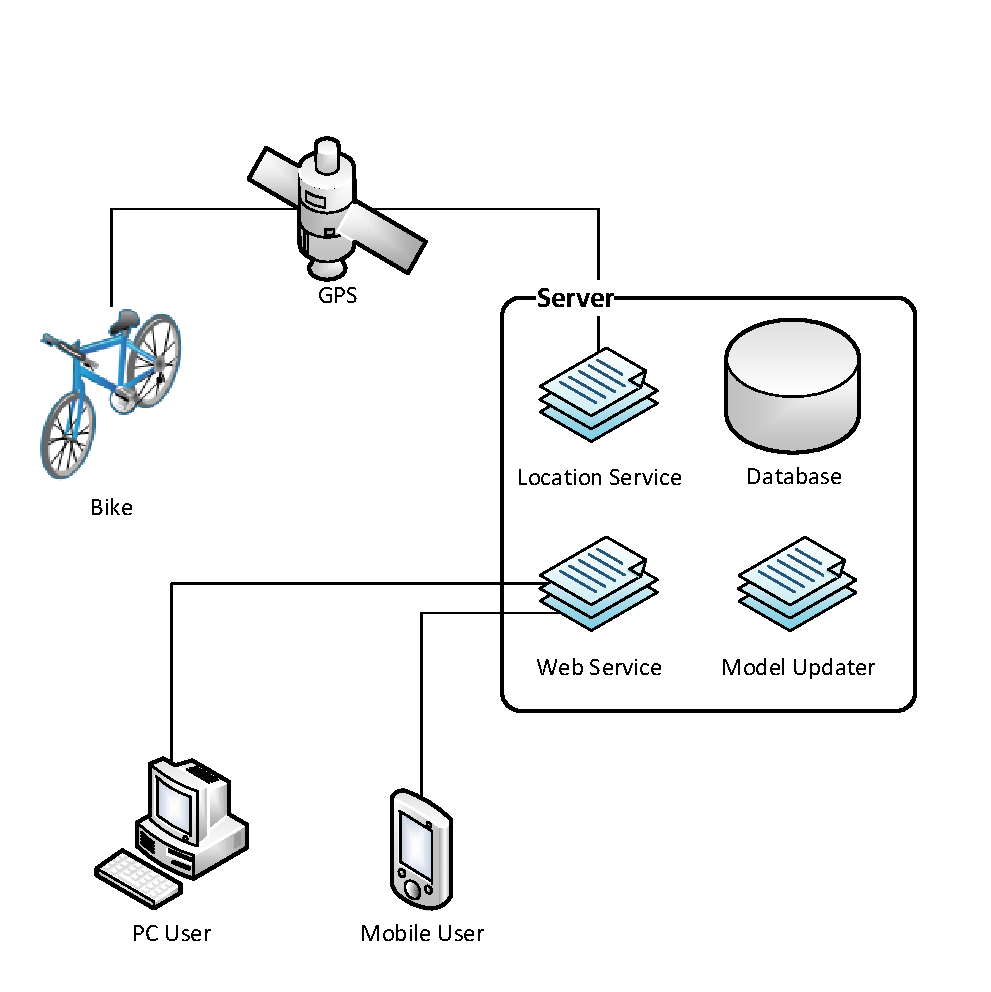
\includegraphics[width=\textwidth, trim={0cm 1cm 2cm 1.5cm}]{our_solution.pdf}
\caption{The overall structure of our solution}
\label{fig:solution_structure}
\end{figure}

The \textit{Location Service} continuously updates the locations of the bikes.
The \textit{Model Updater} uses the stored location data to generate a model used for predictions.
The \textit{Web Service} makes an API available, in order to make platform implementations to make the data available as specified in the requirements.
A web service was chosen as to make the system as available as possible, due to the unspecific target user group.

\subsection{New problems}
In order to develop this system, with the addition of GPS and hotspots, new problems emerge.
The following chapters will focus on the problems:
\begin{itemize}
\item How to define and find hotspots?
\item How to model the usage and use this for predictions?
\item How to make this data available through a web service?
\end{itemize}